\chapter{erster Anhang} \label{anhang1}

Hier können weiter Graphiken oder Ähnliches als Anhang aufgeführt werden. Ebenso sind Untergliederungen der einzelnen Anhang-Kapitel möglich \cite{sundar_exact_2015}

text text text text text text text text text text text text text text text text text text text text text text text text text text text text text text text text text text text text text text text text text text text text text text text text text text text text text text text text text text text text text text text text text text text text text text text text text text text text text text text text text text text text text text text text text text text text text text text text text text text text text 

\section{erste Untergliederung}

text text text text text text text text text text text text text text text text text text text text text text text text text text text text text text text text text text text text text text text text text text text text text text text text text text text text 

\begin{figure}[!ht]
 \begin{center}
  % Requires \usepackage{graphicx}
  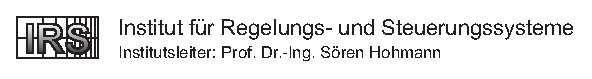
\includegraphics[width=1\textwidth]{irslogo.eps}
  \caption{Abbildung im Anhang}\label{bild_anh}
 \end{center}
\end{figure}

\section{Quellcodes}

Quellcodes lassen sich gut mit dem listings-Paket einbinden, so ist das Einbinden von entsprechend formatiertem Matlab-/C++/etc.-Code ohne Copy/Paste direkt aus der Quellcode-Datei möglich. Und hier noch ein Beispielhafter Matlab Quellcode:

\begin{lstlisting}[caption={Ein wahnsinnig komplizierter Quellcode}]
%% State Space System
asyn.SS = ss(asyn.A,asyn.B,asyn.C,asyn.D);

% Infos über das System
disp('- Informationen über das System -');
% Ordnung des Systems
asyn.n = rank(asyn.A);
disp(['Ordnung des Systems n = ', num2str(asyn.n)]);
% Polstellen
asyn.PS = pole(asyn.SS);
% Nullstellen
asyn.NS = tzero(asyn.SS);
% Beobachtbarkeit
asyn.Ob = obsv(asyn.SS);
if rank(asyn.Ob) == asyn.n
    disp('System vollständig Beobachtbar');
else
    disp('System nicht vollständig Beobachtbar');
end
% Steuerbarkeit
asyn.Os = ctrb(asyn.SS);
if rank(asyn.Os) == asyn.n
    disp('System vollständig Steuerbar');
else
    disp('System nicht vollständig Steuerbar');
end

disp('---------------------------------');
\end{lstlisting}